\section{Team characteristics}

\subsection{Network structure}

\cref{tab:results-team-characteristics-accuracy} shows the \gls{rps} values and accuracy of the team characteristics network. In the evaluation data set, 41.3\% of all matches ended in a home victory.
\begin{table}
    \centering
    \begin{tabulary}{\textwidth}{| L | L || L | L | L || L |}
        \hline
        \multicolumn{2}{| l ||}{\textbf{Hidden layer}}  & \multicolumn{3}{l ||}{\textbf{\gls{rps} values}} & \\\hline
        \textbf{Activation} & \textbf{Size}             & \textbf{Min}  & \textbf{Max}  & \textbf{Mean} & \textbf{Accuracy} \\\hline
        \gls{relu}          & 32                        & 0.0143        & 0.794         & 0.226         & 0.463 \\\hline
        \gls{relu}          & 64                        & 0.00102       & 0.785         & 0.218         & 0.466 \\\hline
        \gls{relu}          & 128                       & 0.0122        & 0.719         & 0.224         & 0.458 \\\hline
        
        \hline
        
        Sigmoid             & 32                        & 0.0130        & 0.737         & 0.217         & 0.460 \\\hline
        Sigmoid             & 64                        & 0.0245        & 0.665         & 0.217         & 0.468 \\\hline
        \rowcolor{correct}
        Sigmoid             & 128*                      & 0.0169        & 0.706         & 0.213         & 0.469 \\\hline
        Sigmoid             & 256*                      & 0.0103        & 0.744         & 0.215         & 0.450 \\\hline
        
        \hline
        
        \Gls{tanh}          & 32*                       & 0.0152        & 0.775         & 0.223         & 0.445 \\\hline
        \Gls{tanh}          & 64*                       & 0.00779       & 0.800         & 0.220         & 0.461 \\\hline
        \Gls{tanh}          & 128**                     & 0.0102        & 0.698         & 0.216         & 0.463 \\\hline
        \Gls{tanh}          & 256**                     & 0.0108        & 0.823         & 0.224         & 0.461 \\\hline
    \end{tabulary}
    \caption{Accuracy of the team characteristics network, with different hidden layer configurations. The row colored green shows the configuration with most promising results.}
    \label{tab:results-team-characteristics-accuracy} 
\end{table}

Using a hidden layer with 128 nodes activated by the sigmoid function yielded the most promising results, and will therefore be used when evaluating the profitability of the team characteristics network. \cref{tab:results-team-characteristics-accuracy-2016-2017} shows the \gls{rps} values and prediction accuracy when evaluating the same configuration over the 2016-2017 season. The network achieved \gls{rps} values similar to the benchmark model the first season. The second season, the network achieved slightly better values.
\begin{table}
    \centering
    \begin{tabulary}{\textwidth}{| L | L | L || L |}
        \hline
        \multicolumn{3}{| l ||}{\textbf{\gls{rps} values}}  &                   \\\hline
        \textbf{Min}    & \textbf{Max}  & \textbf{Mean}     & \textbf{Accuracy} \\\hline
        0.0171          & 0.700         & 0.187             & 0.609             \\\hline
    \end{tabulary}
    \caption{Prediction accuracy of the team characteristics network for the 2016-2017 season of the English Premier League, using the most promising hidden layer configuration.}
    \label{tab:results-team-characteristics-accuracy-2016-2017} 
\end{table}


\subsection{Betting results}

\subsubsection{English Premier League 2015-2016}

\cref{fig:results-team-characteristics-2015-2016-fixed-bet,fig:results-team-characteristics-2015-2016-fixed-return,fig:results-team-characteristics-2015-2016-kelly-ratio,fig:results-team-characteristics-2015-2016-variance-adjusted} show the development of the \gls{roi} generated by the team characteristics network over the English Premier League season 2015-2016.
\begin{figure}
    \centering
    \includegraphics[width=\textwidth]{results/team-characteristics/2015-2016/fixed-bet-10.png}
    \caption{\gls{roi} over the span of the English Premier League season 2015-2016 using the team characteristics network and the fixed bet strategy.}
    \label{fig:results-team-characteristics-2015-2016-fixed-bet}
\end{figure}
\begin{figure}
    \centering
    \includegraphics[width=\textwidth]{results/team-characteristics/2015-2016/fixed-return-10.png}
    \caption{\gls{roi} over the span of the English Premier League season 2015-2016 using the team characteristics network and the fixed return strategy.}
    \label{fig:results-team-characteristics-2015-2016-fixed-return}
\end{figure}
\begin{figure}
    \centering
    \includegraphics[width=\textwidth]{results/team-characteristics/2015-2016/kelly-ratio-10.png}
    \caption{\gls{roi} over the span of the English Premier League season 2015-2016 using the team characteristics network and the Kelly ratio strategy.}
    \label{fig:results-team-characteristics-2015-2016-kelly-ratio}
\end{figure}
\begin{figure}
    \centering
    \includegraphics[width=\textwidth]{results/team-characteristics/2015-2016/variance-adjusted-10.png}
    \caption{\gls{roi} over the span of the English Premier League season 2015-2016 using the team characteristics network and the variance adjusted strategy.}
    \label{fig:results-team-characteristics-2015-2016-variance-adjusted}
\end{figure}

\cref{tab:fig:results-team-characteristics-2015-2016-roi} shows a summary of the \gls{roi} values achieved by the different strategies when used by the team characteristics network. The table shows the final \gls{roi} for the least profitable and most profitable simulations, together with the average final \gls{roi}.
\begin{table}
    \centering
    \begin{tabulary}{\textwidth}{| L || L | L | L |}
        \hline
                            & \multicolumn{3}{l |}{\textbf{Final \gls{roi}}} \\\hline
        \textbf{Strategy}   & \textbf{Min}  & \textbf{Max}  & \textbf{Mean} \\\hline
        Fixed bet           & 0.0010        & 0.54          & 0.21 \\\hline
        Fixed return        & -0.038        & 0.070         & -0.050 \\\hline
        Kelly ratio         & -0.25         & 2.6           &  0.80 \\\hline
        Variance adjusted   & -0.07         & 0.039         & -0.032 \\\hline
    \end{tabulary}
    \caption{Final \gls{roi} values for the four strategies when using the team characteristics network during the 2015-2016 season of the English Premier League. The green colored cell was the most profitable strategy (on average).}
    \label{tab:fig:results-team-characteristics-2015-2016-roi}
\end{table}
      
\cref{fig:results-team-characteristics-2015-2016-odds-prob} shows the bets placed during the 2015-2016 season of the English Premier League. The probabilities are generated by a random instance of the team characteristics network.
\begin{figure}
    \centering
    \includegraphics[width=\textwidth]{results/team-characteristics/2015-2016/odds-prob.png}
    \caption{Offered odds and predicted probabilities for the bets placed during the 2015-2016 season of the English Premier League. The probabilities are generated by the team characteristics network.}
    \label{fig:results-team-characteristics-2015-2016-odds-prob}
\end{figure}
  

\subsubsection{English Premier League 2016-2017}

\cref{fig:results-team-characteristics-2016-2017-fixed-bet,fig:results-team-characteristics-2016-2017-fixed-return,fig:results-team-characteristics-2016-2017-kelly-ratio,fig:results-team-characteristics-2016-2017-variance-adjusted} show the development of the \gls{roi} generated by the team characteristics network over the English Premier League season 2016-2017.
\begin{figure}
    \centering
    \includegraphics[width=\textwidth]{results/team-characteristics/2016-2017/fixed-bet-10.png}
    \caption{\gls{roi} over the span of the English Premier League season 2016-2017 using the team characteristics network and the fixed bet strategy.}
    \label{fig:results-team-characteristics-2016-2017-fixed-bet}
\end{figure}
\begin{figure}
    \centering
    \includegraphics[width=\textwidth]{results/team-characteristics/2016-2017/fixed-return-10.png}
    \caption{\gls{roi} over the span of the English Premier League season 2016-2017 using the team characteristics network and the fixed return strategy.}
    \label{fig:results-team-characteristics-2016-2017-fixed-return}
\end{figure}
\begin{figure}
    \centering
    \includegraphics[width=\textwidth]{results/team-characteristics/2016-2017/kelly-ratio-10.png}
    \caption{\gls{roi} over the span of the English Premier League season 2016-2017 using the team characteristics network and the Kelly ratio strategy.}
    \label{fig:results-team-characteristics-2016-2017-kelly-ratio}
\end{figure}
\begin{figure}
    \centering
    \includegraphics[width=\textwidth]{results/team-characteristics/2016-2017/variance-adjusted-10.png}
    \caption{\gls{roi} over the span of the English Premier League season 2016-2017 using the team characteristics network and the variance adjusted strategy.}
    \label{fig:results-team-characteristics-2016-2017-variance-adjusted}
\end{figure}

\cref{tab:fig:results-team-characteristics-2016-2017-roi} shows a summary of the \gls{roi} values achieved by the different strategies when used by the team characteristics network. The table shows the final \gls{roi} for the least profitable and most profitable simulations, together with the average final \gls{roi}.
\begin{table}
    \centering
    \begin{tabulary}{\textwidth}{| L || L | L | L |}
        \hline
                            & \multicolumn{3}{l |}{\textbf{Final \gls{roi}}} \\\hline
        \textbf{Strategy}   & \textbf{Min}  & \textbf{Max}  & \textbf{Mean} \\\hline
        Fixed bet           & -0.10         & 0.27          & 0.13 \\\hline
        Fixed return        & -0.010        & 0.14          & 0.080 \\\hline
        Kelly ratio         & -0.48         & 1.3           & \cellcolor{correct} 0.70 \\\hline
        Variance adjusted   & 0.041         & 0.21          & 0.12 \\\hline
    \end{tabulary}
    \caption{Final \gls{roi} values for the four strategies when using the team characteristics network during the 2016-2017 season of the English Premier League. The green colored cell was the most profitable strategy (on average).}
    \label{tab:fig:results-team-characteristics-2016-2017-roi}
\end{table}

\cref{fig:results-team-characteristics-2016-2017-odds-prob} shows the bets placed during the 2016-2017 season of the English Premier League. The probabilities are generated by a random instance of the team characteristics network.
\begin{figure}
    \centering
    \includegraphics[width=\textwidth]{results/team-characteristics/2016-2017/odds-prob.png}
    \caption{Offered odds and predicted probabilities for the bets placed during the 2016-2017 season of the English Premier League. The probabilities are generated by the team characteristics network.}
    \label{fig:results-team-characteristics-2016-2017-odds-prob}
\end{figure}


\subsubsection{Summary}

The team characteristics network achieved consistent good results, generating profits over both seasons using the fixed bet and Kelly ratio strategies. The network also generated profits the other strategies the first season.

\cref{fig:results-team-characteristics-2015-2016-odds-prob,fig:results-team-characteristics-2016-2017-odds-prob} show the connection between odds and probabilities predicted by the team characteristics network. The team characteristics network produce far better predictions than any other network. There is, however, a slight tendency to overestimate the probabilities in the lower fifth of the horizontal axis. Over the two seasons, the prediction models won approximately 29.4\% of all bets placed, with an average odds of 3.82.